\chapter{Design and Materials}
\label{chap:design}
\section{Introduction of this chapter}
An \gls{ann}, is a computational model based on the idea that the brain is comprised of interconnected neurons of varying types and connectivity. \gls{ann} also consist of many simple processing elements or "neurons," and can have one or more layers of neurons. Typically, each neuron will have many inputs, they will process the inputs by weighing and summing the input to produce an output (plus one bias), and then a nonlinear activation function is used to produce the last output of the particular neuron. By connecting many layers of these neurons, \gls{ann} can be trained to map complex, nonlinear functions to outputs from raw inputs (pixel intensities or sensor readings) to outputs (class labels or continuous predictions). In this chapter we will set out the basic underpinnings for building , training a neural network, describe why we bother building neural networks and how is it related to our research objective





\section{Introduction to Neural Networks} 
Neural networks now underpin most current state-of-the-art artificial intelligence, in part because of their plausible similarity to human brain information processing. We will identify the basic features of neural networks, and introduce some very rough analogies to help conceptualize the new structures while maintaining appropriate mathematical development. This does indicate a solution that intertwines biology and mathematics that is also flexible and adaptable to convoluted problems in the real world.











\section{Inspiration of Neural Networks}

The first mathematical representation of a neuron was presented by McCulloch and Pitts, who abstracted biological neurons to simplistic binary logic functions. This conceptualization started the trajectory towards artificial neural networks, with the first conceptualizations of computers in the computational models such as the perceptron. It is evident that these models, while development, went from very simple single-layer models to have deep neural networks like we have today that have multiple hidden layers and make complex hierarchically organized representations of input. Artificial neural networks have reached success across a range of computational tasks where they can perform quite complex tasks, including image classifications, natural language processes, and even controlling autonomous systems, even if they are mathematically far less complex than biological organisms.
Biological inspiration continues to be valuable and play an important role in creating artificial neural networks. The human brain has approximately 86 billion neurons that are interconnected, via what we call synapses, and processes information in remarkably efficient and adaptive ways. Neurons transmit signals using extremely complex arrangements of thousands of neuronal pathways. The neuron cell receives signals through dendrites, regardless of organizational type, integrates the signals in the cell body, and transmits the signals through the axon, completing the signal. This process can include both electrical and chemical signaling, which enables our internal environments to response and adapt, learning from our experiences, and then make decisions based on these previously processes experiences. The brain has the ability to continually change, often referred to as 'neural plasticity', is similar to how different learning algorithms work in an artificial network. For instance, synaptic strengths change as a result of stimulation is analogous to how artificial networks update and change their connection weights during training to learn and generalize from data \cite{mcculloch1943logical}.
However, even though artificial neural networks provide some inspiration for biological systems, there are limits to analogy and comparative discussion. Biological neurons all operate in massively parallel, asynchronous, and biochemically dynamic environments, whereas artificial networks perform all over discrete and synchronous computational processes that are made of silicon. Lastly, the efficiency, scalability, and effectiveness of the brain exceeds every artificial system currently available today. Therefore we have to treat artificial neural networks as functioning abstractions that are causing important computational principles to be abstracted in to simplified and tractable forms. Even so, this abstractions has been sufficiently powerful to create systems that appear to have demonstrated robust perception and reasoning abilities across a range of domains.








\section{Why Build Neural Networks?}
The emergence of neural networks as an underlay machine learning techniques owes to three foremost properties that make them especially effective for a wide variety of tasks. First, neural networks have the ability to fit complex and nonlinear functions to a high-degree of accuracy, given enough capacity. This enables neural networks to fit complex relationships in data that often cannot be captured by traditional models. Second, neural networks are able to automatically learn multi-level feature representations directly from raw data, without the require for manual feature engineering, as is the case with traditional methods. The hierarchical feature extraction allows for less domain-specific cleaning, and in many cases better generalization across tasks. Third, well-regularized neural networks have been shown to demonstrate a level of robustness against uncertainty and failure. These systems can tolerate noisy or missing inputs, and minor degradation in internal components can be tolerated without catastrophic loss of performance. As such, the appeal of neural networks for spaceborne AI systems, where at least in part, unexpected environmental changes and limited hardware will be constant challenges. It should be clear that the combination of these properties gives neural networks a flexible, powerful, and robust platform for solving difficult problems on- and off-Earth.















\section{How to Build a Neural Network}
A typical feed-forward network is built from three building blocks:


    \subsection{Artificial Neuron}  An artificial neuron is designed to mimic the behavior of a biological neuron and is composed of three essential components:
    \begin{itemize} 
        \item \textbf{Inputs} ($x_1, x_2, \ldots, x_n$): The individual numbers shown here are just values representing different features inferred possibly from the original data like pixel intensity in an image in the context of computer vision or measurement readings taken in the context of an IoT device. Each input has some information and together they form something more meaningful that is an aggregation of the original data. 
        \item \textbf{Weights} ($w_1, w_2, \ldots, w_n$):The parameters reviewed in the preceding section indicate the relative degree of importance of each input. During training, the weights assigned to the inputs will be changed by the network to learn the appropriate comparative weightings in order for the best representation of a pattern and hence, the appropriate response.
        \item \textbf{Activation Function} ($f$): This function is responsible for determining whether the neuron will activate (or "fire") and send its signal to all the downstream neurons. Early models used binary step functions that made specific decisions. Increasingly current networks use a smooth, non-smooth function to extract finer patterns from the data, such variables index for example, ReLU \cite{nair2010rectified} functions.
    \end{itemize}
    The output of an artificial neuron is computed by: 
    \begin{equation}  y = f\left(\sum_{i=1}^n w_i x_i + b\right) \end{equation} 
    In this equation, $b$ is the bias term which allows you to shift the function horizontally which helps it to better fit the data. This simple equation is the basis for neural networks: it allows the neural networks to learn rich maps from input to output.


    \subsection{Layer Structure}
    Although a single neuron can only solve relatively simple, linearly separable tasks, the complexities of many real-world problems require more sophisticated types of decision boundaries. Thus, neurons are joined to each other to create multi-layered structures, typically referred to as neural networks. A fully connected neural network will typically consist of:
    \begin{itemize} 
        \item \textbf{Input Layer}: The layer of input receives the raw data directly. An image, for example, is often flattened into a one-dimensional vector like 784 inputs, for a 28×28 pixel image. 
        \item \textbf{Hidden Layers}: The hidden layers iteratively extract and transform features using nonlinear transformations. Each hidden layer builds its representation of the data, where the use of the term “deep learning” comes into usage due to the many hidden layers.  
        \item \textbf{Output Layer}: The output layer transforms the features observed from the hidden layers into either probabilities or continuous values. 
    \end{itemize}
   Apart from the basic components, additional complex architectures, such as convolutional layers (used for image data), and recurrent layers (used for sequence data), add more ability to neural networks for an even larger space of problems.


    \subsection{Activation Functions}
    Activation functions play a critical role in neural networks by introducing the nonlinearity necessary to approximate complex, high‐dimensional mappings. The most common choice, the Rectified Linear Unit (ReLU), defined as 
    \[
    \mathrm{ReLU}(z)=\max(0,z),
    \]
    combines computational simplicity with a constant gradient for \(z>0\), greatly mitigating the vanishing‐gradient problem in deep architectures \cite{nair2010rectified}. Nonetheless, ReLU can suffer from “dying” neurons that never activate; to address this, variants such as Leaky ReLU or Parametric ReLU allow a small, learnable slope for negative inputs. Traditional sigmoid 
    \[
    \sigma(z)=\frac{1}{1+e^{-z}}
    \]
    and hyperbolic tangent 
    \[
    \tanh(z)=\frac{e^z-e^{-z}}{e^z+e^{-z}}
    \]
     functions have traditionally been the workhorse functions but generally saturate for larger  \(|z|\)values, and gradients still vanish for some of the earlier layers. More recent smooth activations (often still classified as sigmoidal)—including Swish or GELU—stay positive across the real line and generally have faster convergence and higher accuracy on big data tasks. Ultimately, the decision of which activation function to use balances gradient flow, representational capacity, and computational cost; the impact on training dynamics and final performance can be significant.  













\section{How to train a Neural Networks}

    \subsection{Data Preparation and Mini-Batching}
    Before any learning can take place, there is a prior step to preprocessing the raw input data (including your image files and sensor readings). This is done to normalize the features you will be comparing so that they are on a comparable scale. In most preprocessing methods, for each feature, the values are normalised or standardised so that their resulting values have approximately zero mean and unit variance, or rescaling the range of pixel intensities. After normalising the data, the larger dataset is further split into smaller, randomly selected subsets which we refer to as mini-batches. When training a network, the use of mini-batches, rather than the entire dataset, has its tradeoffs. Each update to the networks parameters is based on a sufficient number of examples to give a clear signal. But the updates come frequently enough, that the time saved in finding the minima of the cost function is still an advantage to the learning process, in terms of a low probability for the algorithm to become stuck.
    
    
    
    \subsection{Forward Propagation}
    During a common forward pass of a deep neural network, in the style of Figure~\ref{fig:forward-loss-backprop}, the input vector is passed to the input layer, the input layer output is then passed to non-linear function (NLF1) to impart the necessary non-linearities for the model. The output of the previous layer is followed by a linear transformation which is passed to the first hidden layer. Once again, processing occurs in the hidden layer and its output is passed to another non-linear function (NLF2). The stream of processing continues as a linear transformation followed by a non-linear activation; i.e., the input is passed from layer to layer through an ordered series of linear transformation and non-linear activations. Finally, the output of the last hidden layer is passed through the output layer, activating the output layer to produce a vector of logits, each representing a real-valued output over the possible classes. The logits may then be change to class probabilities over the possible classes by a softmax function or other methods, depending on the task.
    
    \subsection{Loss Computation}
    The output layer logits are turned into a probability distribution using a softmax transformation, which exponentiates each logit, and divides that by the sum of the exponentials. This gives us non-negative values that sum to one (the "new output") as seen in Figure ~\ref{fig:forward-loss-backprop}. These probabilities are now used in conjunction with the true labels in the loss node using cross-entropy loss. The probability of a correct classification is inversely proportional to the loss value, meaning that when the probability is low, the losses will be larger, and when they are high, the losses will be low. This scalar loss value indicates how close the model's prediction is to the true targets.

    \begin{figure}[H]
      \centering
      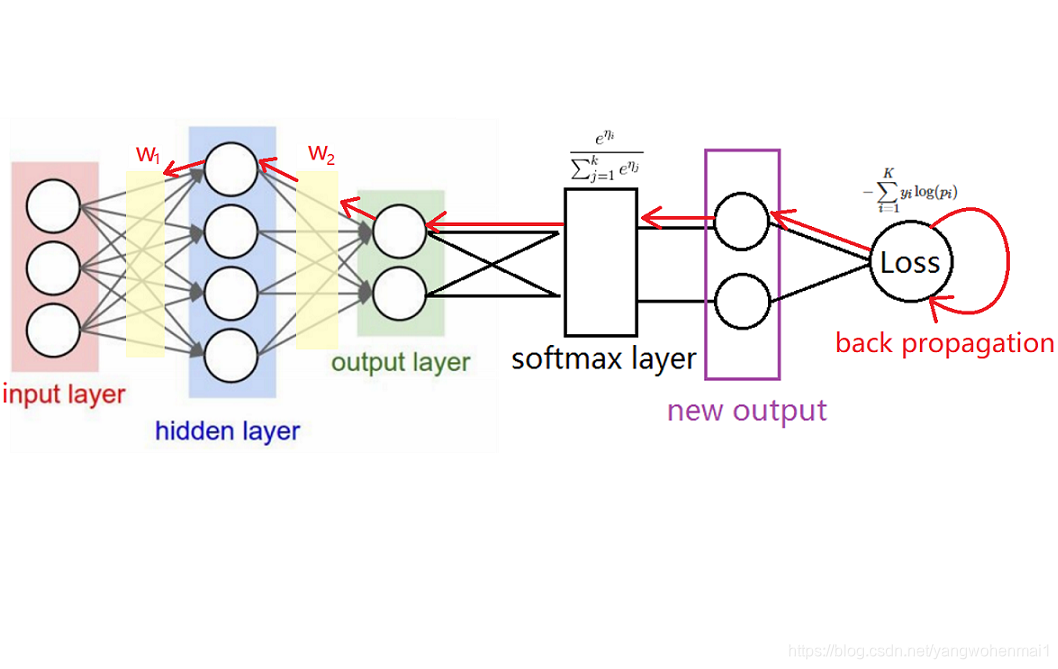
\includegraphics[width=0.45\textwidth]{images/forward&backward_propagation.png}
      \caption{Illustration of forward propagation, softmax + loss, and backpropagation.}
      \label{fig:forward-loss-backprop}
    \end{figure}
    
    \subsection{Backpropagation and Gradient Calculation}
    Once the loss is calculated, backpropagation can proceed. Backpropagation asks how a small change in each upstream quantity somehow nicknamed softmax inputs, then (softmax) output-layer activations, (softmax) hidden-layer activations, and last the parameters' weights (W\_2) and (W\_1)) can impact the loss. We are able to calculate this from the loss node. As such, it computes gradients for every weight in the network, through the manipulation of the reverse chain rule. These gradient values were then passed on to an optimizer (like stochastic gradient descent) which was able to update the parameters and weights such that in its future forward passes the total loss was minimized.

    
    \subsection{Parameter Update and Optimization}
    After the calculations of the gradients, the network now has to update its parameters, which can be done by adjusting the parameters in whichever direction will decrease the loss. How do you determine which direction to go? The gradient points the direction of the next step and a tunable number called the learning rate provides the magnitude of the movement, or how aggressive or conservative each step is towards minimizing the loss. In machine learning, simple stochastic gradient descent is a straightforward way to update the parameters of a function where you take a fixed step size for each parameter. More sophisticated optimizers such as momentum, AdaGrad, RMSProp and Adam actually tune the step sizes based on the history of gradients, allowing for improved convergence of model stability and speed.
    
    \subsection{Training Loop and Convergence Criteria}
    The complete training process is characterized by repeating the following set of steps: selecting a mini-batch, performing forward propagation, computing loss, performing backpropagation, and moving weights for each mini-batch in the data set. Completing a batch is one epoch. During the training process and after each epoch, we reshuffle the data to avoid the models learning patterns from a random batch order. Performance is usually reported after each epoch on completely separate validation data, which we will use to track generalization. Training continues for what seems to be an eternity until we meet some stopping criteria. This may be true when we stop because the validation loss does not decrease for a certain number of epochs, or early stopping. Or the training stops when the validation data reaches some target accuracy. After which, we are done training, and the parameters have been optimally set to represent new or unseen data to classify accordingly.
    
    \subsection{Dropout Regularization}
    The entire training process consists of repeating a series of steps, which include selecting a mini-batch, performing forward propagation, computing loss, performing backpropagation, and updating the weights for all mini-batches in the dataset. Completing one batch is called one epoch. In the first layer, the use of each neuron (with in and out connections) is dropped, proportionally to a fixed probability (p) for each training example, which is typically 0.5 for hidden layers. The remaining active neurons must then learn a more efficiently robust distributed representation -- since they no longer have specific units that are partnered with other specific units.
    Dropout is, by definition, the process of limiting the ability of any one neuron to dominate the response of the neural network, by providing redundancy with features distributed across parallel pathways. Experience has shown this enhances generalisation and reduces the need for any other forms of regularization, while also expediting convergence by increasing stability in the face of the inherent variability in the surface to be optimized. It is important to note here that always think about each aspect throughout experimental design. At this point, it has trained the model and fitted appropriate parameters in order to achieve a level of generalization performance on new or unseen data. 
    Throughout our experimental regime, we have used dropout at each hidden layer (as a regularizer in response to overfitting small, specific datasets), with (p = 0.5) dropout regularization but have not applied dropout to an explicit mechanism of fault tolerance against radiation-induced faults. Although random dropping of neurons has been shown to inadvertently make DNNs more resilient to random perturbations, the intention of dropout is not to improve the robustness of DNNs in respect to bit-flips. It is to reduce the size of an \gls{dnn} (through pruning and quantitation) and perform systematic studies of error-injects to characterize fault-tolerance.



\section{How should we choose our model?}

Knowledge of the basic principles behind neural networks is necessary before evaluating the most appropriate neural network model you need for your project. Also, to improve the confidence in the experiment, this study additionally chose a 'large model' and a 'small model' for comparison or evaluation purposes.

    \subsection{"Large Model": VGG-16}
    The "large model" was determined to be the classic VGG-16 network due to the following reasons:
    \begin{itemize}
      \item \textbf{Depth and Capacity}: VGG-16 is characterized by 16 layers of learnable parameters, with an approximate total of 138 million parameters. This configuration enables the model to capture complex spatial features and high-level semantic information.
      \item \textbf{Simple Structure}: All convolutional layers utilize $3\times3$ convolutional kernels, and the network possesses a rigid "stacked" configuration, thereby enabling structured pruning and quantization optimization.
      \item \textbf{Well Validated}: VGG-16 has been extensively validated in a variety of visual tasks with regard to accuracy and generalization ability, and it possesses abundant pre-trained weights available for fine-tuning.
    \end{itemize}
    
    \subsection{"Small Model": CCDF}
    In this paper, we described a light-weight model architecture using complementary cumulative distribution functions (CCDF). The use of CCDF model is considered a "small model" in that it contains far fewer learnable parameters (generally fewer than 5 million total) compared to traditional convolutional networks, which is one of its key advantages for resource-limited applications.








\section{Why and How Compress Models}
    \subsection{Inference Efficiency}
    Modern \gls{dnn} frequently require billions of \gls{flops} for a single forward pass, which directly results in high latency when executed on constrained hardware. The elimination of filters or channels that contribute marginally to final accuracy can result in a reduction of both the number of operations and the size of intermediate activations. This results in reduced inference times, which is paramount when a real-time response is imperative onboard a spacecraft. Furthermore, this approach diminishes the total memory footprint, thereby facilitating the deployment of the system on devices with limited memory capacity, such as those with only a few megabytes of RAM.
    
    \subsection{Power and Energy Savings}
    All arithmetic operations and memory accesses for neural networks burn energy, and often in battery- or solar-powered space platforms, energy is the most constrained resource. Although it was established that structured pruning can save computational costs and allow a higher fraction of the model to fit in low-power on-chip memory (as opposed to expensive external DRAM), rather substantial evidence has been presented demonstrating that savings such as this can provide longer mission durations or free up the energy to pursue different subsystems (e.g. communications and navigation), and to possibly allow AI-based tasks in energy collision environments.

    \subsection{Reduced‐Precision Inference}
    To achieve further model size reduction and speed up computation beyond pruning, full-precision (32-bit) weights and activations are replaced with lower-bit representations, typically 8-bit integers. The process is called quantization, in which floating‐point parameters are mapped to the nearest value in a discrete fixed code book. This makes possible the use of fast integer arithmetic units instead of required more power‐hungry floating point pipelines. In practice, the linear weights ranges are scaled to the (-128,127) range while keeping per-channel scaling factors for scaling and dynamic range. Therefore, the result is a 4x lower memory size of each parameter. The aforementioned reduction in memory has three effects: firstly, it results in a reduction in memory consumption; secondly, it improves the compute throughput of specialized hardware; and thirdly, it reduces energy usage.
    
    \subsection{Memory and Bandwidth Savings}
    The evidence is clear that lower bit-width representations can greatly decrease the amount of data that has to move from off-chip memory. It has been shown that because each weight is only one byte instead of four bytes, models can routinely have the ability to fit completely in on-chip SRAM or cache. This avoids the expensive DRAM accesses altogether. This has been shown to reduce both latency - critical for real-time decision loops in spacecraft navigation or anomaly detection - and dynamic power consumption, thereby prolonging missions on solar- or battery-operated platforms.
    
    \subsection{Radiation‐Modeled Bit‐Flip Injection}
    Random bit-flips were injected into the quantized weight tensors during inference to simulate \gls{seu} from cosmic radiation. The faults were added at a steady rate of one bit-flip per 100 \gls{flops} with the aim of approximately emulating the statistical properties of radiation-induced errors expected in space. This allows for the development of realistic fault models without having to change hardware or have the expense and complications of a dedicated radiation testing facility. It also captures the inherently stochastic effect of high-energy particle strikes on memory cells.











\section{Relating to Our Research Objective}
 The chapter reviewed the areas that have helped shape the embrace of neural networks as a viable technologies subjective to different ways of utilizing neural networks to approximate universal functions, automated feature learning and fault tolerance. The chapter concluded with the essential building blocks of a feed-forward network: artificial neurons, layers of neurons and activation functions.


The second portion of the seminar involved a detailed exploration of the entire end-to-end training process for a neural network. There are numerous steps comprising the training process which includes data normalization, mini-batches, forward and backward propagation, loss calculation, parameter fitting and regularization to reduce the possibility of overfitting using dropout. Following this, we followed with a discussion of model selection processes which extended to the selection of a 'large' VGG-16 model because of its depth, its relatively simple 3x3 convolutional structure and its impressive validation accuracy. We subsequently chose a 'small' CCDF model which shall prove useful in terms of the global average pooling and CCDF-based design with remarkable parameter efficiency and optimal levels of built-in robustness evaluation strategy. 


The justifications for model compression were lastly discussed - including the benefits to using structured pruning for increased inference time efficiency, energy efficiency and physical hardware compatibility; quantization for reduced memory space efficiency and an accelerated integer math advantage; and introduced radiation-modeled bit-flips after experiencing a space (on-orbit) single event upset. In our research we strive to characterize trade-off associated with structure-driven FLOPS reduction and classification accuracy and simultaneously simulate the effects of on-orbit radiation fault. The investigation was initiated with the aim to determine knowledge that could support the development of lightweight, yet high levels of capacity neural networks for space-based applications.
